%!TEX root = thesis.tex

\chapter{Results: Priority and Severity} % (fold)
\label{cha:results_priority_and_severity}

In this chapter, the first research question and the accompanying hypothesis are investigated, as defined in Section~\ref{sec:research_questions}:

\vspace{\baselineskip}
\questiona{}
\vspace{\baselineskip}

\noindent
In order to answer this question, certain relationships need to be present in the data. To research if these relationships are present, the following hypotheses are stated:

\vspace{\baselineskip}
\hypaa{}

\vspace{\baselineskip}
\hypab{}

\vspace{\baselineskip}
\hypac{}

\vspace{\baselineskip}
\hypad{}

\vspace{\baselineskip}
\hypae{}

\vspace{\baselineskip}
\hypaf{}

\vspace{\baselineskip}

\section{Overview} % (fold)
All investigations in this chapter are split into three parts: 
\begin{inparaenum}[(1)]
\item \textbf{results}, describing the direct results of the study and showing some descriptive statistics,
\item \textbf{analysis}, analysing the results of the study, and
\item \textbf{conclusions}, which evaluates the hypotheses.
\end{inparaenum}

In Section~\ref{sec:analysis_of_priority_and_severity_related_to_the_presence_of_a_stack_trace}, a possible relation between priority (and severity) of bug reports with the presence of one or more stack traces is investigated. Section~\ref{sec:analysis_of_priority_and_severity_related_to_package_size} investigates if the priority and severity of a bug report tend to be higher if the corresponding packages for the stack trace(s) in the bug report have a larger size. The same investigation is performed on class level in Section~\ref{sec:analysis_of_priority_and_severity_related_to_lines_of_code}.

Finally, all results found in the previous mentioned sections are summarised in Section~\ref{sec:priosev-summary_of_results}.
% section overview (end)

\section{Analysis of priority and severity related to the presence of a stack trace} % (fold)
\label{sec:analysis_of_priority_and_severity_related_to_the_presence_of_a_stack_trace}
When a stack trace is present, a bug triager might be able to identify the location of a bug in source code more easily. This way, it might be also easier to assign a representative priority and severity to the bug report (i.e., less bugs with default priority and severity).

As can be seen in Tables \ref{tab:priority} and \ref{tab:severity}, some small differences exists between the presence of a stack trace versus priority, as well as for the presence of a stack trace versus severity. For example, around 2.5\% more bug reports with priority higher than normal are counted when a stack trace is present. Also, the number of bug reports with severity higher than normal shows a 7.0\% increase.

In this section, we investigate if there is a relation between priority versus presence of a stack trace. The same investigation is performed for severity. In short, the following two hypotheses of research question R1 are discussed: 

\vspace{\baselineskip}
\hypaa{}

\vspace{\baselineskip}
\hypab{}
\vspace{\baselineskip}

\subsection{Results} % (fold)
The count results for priority can be found in Table~\ref{tab:prio-counts}. It shows, for both the two projects as well for the overall situation, the number of bug reports for each priority. A distinction is made between bug reports with a stack trace present, and bug reports without a stack trace in the comments. In Table~\ref{tab:sev-counts}, the same data is presented for the severity.

\begin{table}[!ht]\footnotesize
	\centering
	\begin{tabular}{lrrrrrrr}
		\toprule		
		 & \texttt{jdt.debug} &  & \texttt{jdt.core} &  & overall & \\
		priority & w/o trace & w/ trace & w/o trace & w/ trace & w/o trace & w/ trace\\
		\midrule
		P1 (high) & 380 & 45 & 153 & 21 & 533 & 66\\
		P2 & 623 & 51 & 344 & 22 & 967 & 73\\
		P3 (default) & 6,056 & 496 & 12,190 & 769 & 18,246 & 1,265\\
		P4 & 142 & 6 & 78 & 1 & 220 & 7\\
		P5 (low) & 14 & 0 & 290 & 3 & 304 & 3\\
		\bottomrule
	\end{tabular} 
	\caption{Number of bug reports for each priority.}
	\label{tab:prio-counts}
\end{table}

\begin{table}[!ht]\footnotesize
	\centering
	\begin{tabular}{lrrrrrrr}
		\toprule		
		 & \texttt{jdt.debug} &  & \texttt{jdt.core} &  & overall & \\
		severity & w/o trace & w/ trace & w/o trace & w/ trace & w/o trace & w/ trace\\
		\midrule
		Blocker & 61 & 9 & 136 & 23 & 197 & 32\\
		Critical & 239 & 28 & 352 & 40 & 591 & 68\\
		Major & 433 & 59 & 1,049 & 121 & 1,482 & 180\\
		Normal & 4,809 & 477 & 9,176 & 604 & 13,985 & 1,081\\
		Minor & 256 & 11 & 563 & 17 & 819 & 28\\
		Trivial & 106 & 3 & 140 & 0 & 246 & 3\\
		\bottomrule
	\end{tabular} 
	\caption{Number of bug reports for each severity.}
	\label{tab:sev-counts}
\end{table}
% subsection results (end)

\subsection{Analysis} % (fold)
To test whether there is an association between priority and presence of a stack trace (and between severity and presence of a stack trace), a statistical test of independence is performed. The null hypothesis of such a test states `there is no association between two variables', where the alternative hypothesis states `the two variables are associated'. Since the data under test is categorical data (i.e., count data), a chi-squared test is used (see Section~\ref{sub:chi_squared_test}). In total, a number of six chi-squared tests are executed; tests for \texttt{jdt.debug}, \texttt{jdt.core} and the overall situation, for both priority and severity. 

The validity of a chi-squared test depends on the sample size of the whole dataset and the \emph{expected} theoretical cell counts. For all six tests, the chi-squared approximation is adequate.

The results of the six association tests can be found in Table~\ref{tab:chi2}.

\begin{table}[!ht]\footnotesize
	\centering
	\begin{tabular}{lrrl}
		\toprule		
		association & $\chi^2$ & $p$ & \\
		\midrule
		priority -- \texttt{jdt.debug} & $\chi^2(4, N=7,813) = 9.12$ & $0.058$ & \\
		priority -- \texttt{jdt.core} & $\chi^2(4, N=13,871) = 27.63$ & $< 0.001$ & ***\\
		priority -- overall & $\chi^2(4, N=21,684) = 40.22$ & $< 0.001$ & ***\\
		\midrule
		severity -- \texttt{jdt.debug} & $\chi^2(5, N=6,491) = 20.23$ & $0.001$ & *** \\
		severity -- \texttt{jdt.core} & $\chi^2(5, N=12,221) = 76.34$ & $< 0.001$ & *** \\
		severity -- overall & $\chi^2(5, N=18,712) = 86.49$ & $< 0.001$ & ***\\
		\bottomrule
	\end{tabular} 
	\caption{Chi-squared test results. Format: $\chi^2(df, N=n)$, with $df$ the degree of freedom, and $n$ the number of counts.}
	\label{tab:chi2}
\end{table}

\subsubsection{Priority} % (fold)
Overall, 90\% of all bug reports is assigned the default priority P3. For each separate data set (\texttt{jdt.debug} and \texttt{jdt.core}), the default priority P3 is respectively 84\% and 93\%. For \texttt{jdt.debug}, around 14\% of all bugs get assigned a higher than normal priority, compared to only 4\% for \texttt{jdt.core}. 

When the overall data set is split into two groups --- bug reports with and without one or more stack traces --- some differences can be spotted. The percentage of bugs that get assigned priority P3 deceases with 1.0\% for \texttt{jdt.debug} and increases with 0.8\% for \texttt{jdt.core}. For \texttt{jdt.debug}, 13.9\% of all bug reports without a stack trace get assigned a higher than normal priority, compared to 16.0\% for bug reports that include a stack trace, resulting in an increase of 2.1\%. For \texttt{jdt.core}, an increase of 1.5\% is shown, going from 3.8\% for bug reports without a stack trace, to 5.3\% for bug reports that include a stack trace. 

As expected, the opposite result is visible in the number of bug reports with a lower than normal priority. For \texttt{jdt.debug}, a decrease of 1.2\% is shown, and for \texttt{jdt.core} a decrease of 2.3\%.

Despite these numbers, the chi-squared test does not show a significant result for \texttt{jdt.debug}, accepting the hypothesis that there is no association between priority and the presence of a stack trace. This can be explained by looking at the contribution of each association to the overall chi-squared statistic\footnote{see Section~\ref{sub:chi_squared_test}}. Only the particular association between \texttt{jdt.debug} and P1 shows a significant difference.

For \texttt{jdt.core}, the chi-squared test does show a significant result, rejecting the null hypothesis and giving evidence that there is an association between the variables (but not \emph{which} association). When looking at the contribution of each association to the overall chi-squared statistic, P1 and P5 show a significant difference, which can be attributed to the increase of 1.4\% for P1 and decease of 1.8\% for P5.

For the combined data set, a significant result for the chi-square test is shown. Most attribution for this is, again, for the increase of P1 and decrease of P5.
% subsubsection priority (end)

\subsubsection{Severity} % (fold)
Overall, 80\% of all bug reports is assigned the default severity `normal' and around 9\% is considered a `major' bug report. Compared to the priority attribute, around 10\% less bug reports is assigned the default severity. Overall, 14\% of all bug reports get assigned a higher than normal severity, and around 6\% a less than normal severity. These numbers are similar for the \texttt{jdt.debug} and \texttt{jdt.core} data sets.

When the overall data set is split into two groups --- bug reports with and without one or more stack traces --- some differences can again be spotted. The percentage of bugs that get assigned severity `normal' deceases with 5.4\% for \texttt{jdt.core}, but does not change much for \texttt{jdt.debug}. For \texttt{jdt.debug}, 12.3\% of all bug reports without a stack trace get assigned a higher that normal severity, compared to 16.4\% for bug reports that include a stack trace. This results in an increase of 4.1\%. For \texttt{jdt.core}, an increase of 9.4\% is shown, going from 13.5\% for bug reports without a stack trace, to 22.9\% for bug reports that include a stack trace. 

This increase in higher severity bug reports that include a stack trace is also reflected in the number of bug reports with a lower than normal severity. For \texttt{jdt.debug}, a decrease of 3.7\% is shown, for \texttt{jdt.core} a decrease of 4.0\%.

The chi-squared tests show a highly significant result for \texttt{jdt.debug}, \texttt{jdt.core} and the overall data set, rejecting the hypothesis that there is no association between severity and the presence of a stack trace. This can be explained by looking at the contribution of each association to the overall chi-squared statistic. The attribution of each value for a bug report with a stack trace is significant, except for the `normal' severities and `blocker' and `critical' severities in the case of \texttt{jdt.debug}.
% subsubsection severity (end)
% subsection analysis (end)

\subsection{Conclusions} % (fold)
As can be seen in Tables \ref{tab:priority} and \ref{tab:severity} and their graphical representations in Figure \ref{fig:priority} and \ref{fig:severity}, some differences can be noted between bug reports with and without a stack trace. The results of the chi-square test in Table~\ref{tab:chi2} also shows some significant results.

In \cite{Bettenburg2007} and \cite{Zimmermann2010}, it is shown that the presence of a stack trace is a sign of quality of a bug report. High quality bug reports are likely to get more attention from developers and triagers, which might also be why they get assigned a more representative priority and severity, instead of the default value.

\subsubsection{Priority} 
For \texttt{jdt.debug}, no evidence for an association between priority and presence of a stack trace is found, but the number of high priority bug reports does increase and the number of low priority bug reports does decrease when a stack trace is present. On the other hand, for \texttt{jdt.core} and the overall data set, evidence is found for an association between priority and the presence of a stack trace. When investigating the contribution of each association\footnote{Please refer to Section~\ref{sub:chi_squared_test}} to the overall chi-squared statistic and the bar charts, some evidence is found that bug reports with a stack trace are more common assigned priority P1 (2.6\% versus 4.6\% for the overall situation). Also, the number of low priority bugs decreases when a stack trace is present (2.6\% versus 0.7\% for the overall situation). This gives enough evidence to at least partially accept hypothesis High:

\vspace{\baselineskip}
\hypaa{}
\vspace{\baselineskip}

\noindent
Schr\"{o}ter \emph{et al.} \cite{Schroter2010} showed that stack traces are valuable pointers to points of interest in the source code. We also showed that stack traces can be used as pointers to other bug reports. This way, it might be easier for a triager to assess a better priority for the bug report, since the possible costs for a fix might be easier to determine (by inspecting source code and related bugs).

\subsubsection{Severity}
For all data sets, evidence is found for an association between severity and the presence of a stack trace. When investigating the contribution of each association to the overall chi-squared statistic and the bar charts, the number of bug reports with a higher than normal severity increases when a stack trace is present (13.1\% versus 20.1\% for the overall situation). Also, the number of bug reports with a lower than normal severity decreases when a stack trace is present (6.1\% versus 2.2\% for the overall situation). This gives enough evidence to accept hypothesis H1.2:

\vspace{\baselineskip}
\hypab{}
\vspace{\baselineskip}

\noindent
In \cite{Schroter2010}, it is showed that in up to 60\% of fixed bug reports, the bug is actually fixed in one of the methods mentioned in a stack trace. This means that when a stack trace is present in the bug report, a triager might be able to perform a better assessment of the severity of a bug by inspecting the source code.
% subsection conclusions (end)

% section analysis_of_priority_and_severity_related_to_the_presence_of_a_stack_trace_in_a_bug_report (end)

\section{Analysis of priority and severity related to package size} % (fold)
\label{sec:analysis_of_priority_and_severity_related_to_package_size}
When one or more stack traces are present in comments of a bug report, it is possible to relate each bug report to one or more source packages. A larger package size might point to a more important subsystem of the software, hence to a higher priority or severity of a bug. In this section, it will be investigated whether there is a relation between the priority (and severity) of a bug report and the size of the related packages references in stack traces in this bug reports.

The \emph{size} of a package is not bound to a single evident definition. Three possible definitions are investigated in this section:

\begin{enumerate*}
	\item number of classes (NOC)
	\item total lines of code of associated classes (SUMLOC)
	\item (arithmetic) mean of lines of code of associated classes (AVGLOC)
\end{enumerate*}

Some descriptive statistics for package size can be found in Section~\ref{sec:descr:package_size}.

\subsection{Results} % (fold)
For each bug report with a stack trace, all associated packages are determined, which in turn have the above mentioned size metrics (when their associated classes can be found in the source code repository). A bug report can have multiple stack traces, and a stack trace can have multiple associated packages. This results in a list of pairs \emph{(report, package)}. It is possible that the same stack trace is mentioned multiple times in a bug report (for example in a quoted message). Also, a package can be mentioned multiple times in a stack trace.

In order to make sure these duplicates do not affect the statistics, only unique pairs \emph{(report, package)} are considered. The pair-counts for all issues under investigation can be seen in Table~\ref{tab:package-tuple-counts}. As can be seen, default values P3 and `normal' are most commonly used.

\begin{table}[!ht]\footnotesize
	\centering
	\begin{tabular}{lrrrrrr}
		\toprule
		 & \texttt{jdt.debug} & \texttt{jdt.core} & overall\\
		\midrule
		P1 & 4 & 5 & 9\\
		P2 & 19 & 10 & 29\\
		P3 & 332 & 1,149 & 1,481\\
		P4 & 5 & 0 & 5\\
		P5 & 0 & 9 & 9\\
		\midrule
		Total & 360 & 1,173 & 1,533\\
		\midrule
		\\
		Blocker & 0 & 57 & 57\\
		Critical & 7 & 56 & 63\\
		Major & 39 & 180 & 219\\
		Normal & 308 & 859 & 1,167\\
		Minor & 0 & 19 & 19\\
		Trivial & 0 & 0 & 0\\
		\midrule
		Total & 354 & 1,171 & 1,525\\
		\bottomrule
	\end{tabular} 
	\caption{Unique \emph{(report, package)} pair-counts.}
	\label{tab:package-tuple-counts}
\end{table}
% subsection results (end)

\subsection{Analysis} % (fold)
In order to investigate whether there is a relation between priority (or severity) and package size, a pairwise comparison of the median values of each data set is performed. For priority, P1 and P2 are compared, P2 and P3, et cetera. For severity, `blocker' and `critical' are compared, `critical' and `major', et cetera.

As can be seen in Table~\ref{tab:package-tuple-counts}, the number of data points for non-default priority is very low, which is consistent with the research performed in \cite{Lamkanfi2010}, who found that most bug reports get assigned the default value for priority and severity. This means it is not possible to thoroughly investigate the hypothesis. However, for severity, a analysis can be made in the case of \texttt{jdt.core}. With this data set, three comparisons can be made (`blocker' versus `critical', `critical' versus `major', `major' versus `normal'). Using these three comparisons, a possible relationship between the two dimensions priority (or severity) and package size can be shown.

The box plots for the data sets for all three size metrics under investigation is depicted in Figure~\ref{fig:packages-box-sevcore}. Some descriptive statistics are shown in Table~\ref{tab:package-sev-stats}. For all minimum and maximum values, a lot of similar numbers can be seen for the lines-of-code metric and number of classes metrics. This is probably due to some specific files that are quite common is stack traces. For NOC, a decrease in median and mean values is seen when the severity becomes higher. The same applies to SUMLOC, but no changes can be spotted for AVGLOC.

\begin{figure}
        \begin{subfigure}[b]{0.5\textwidth}
                \centering
                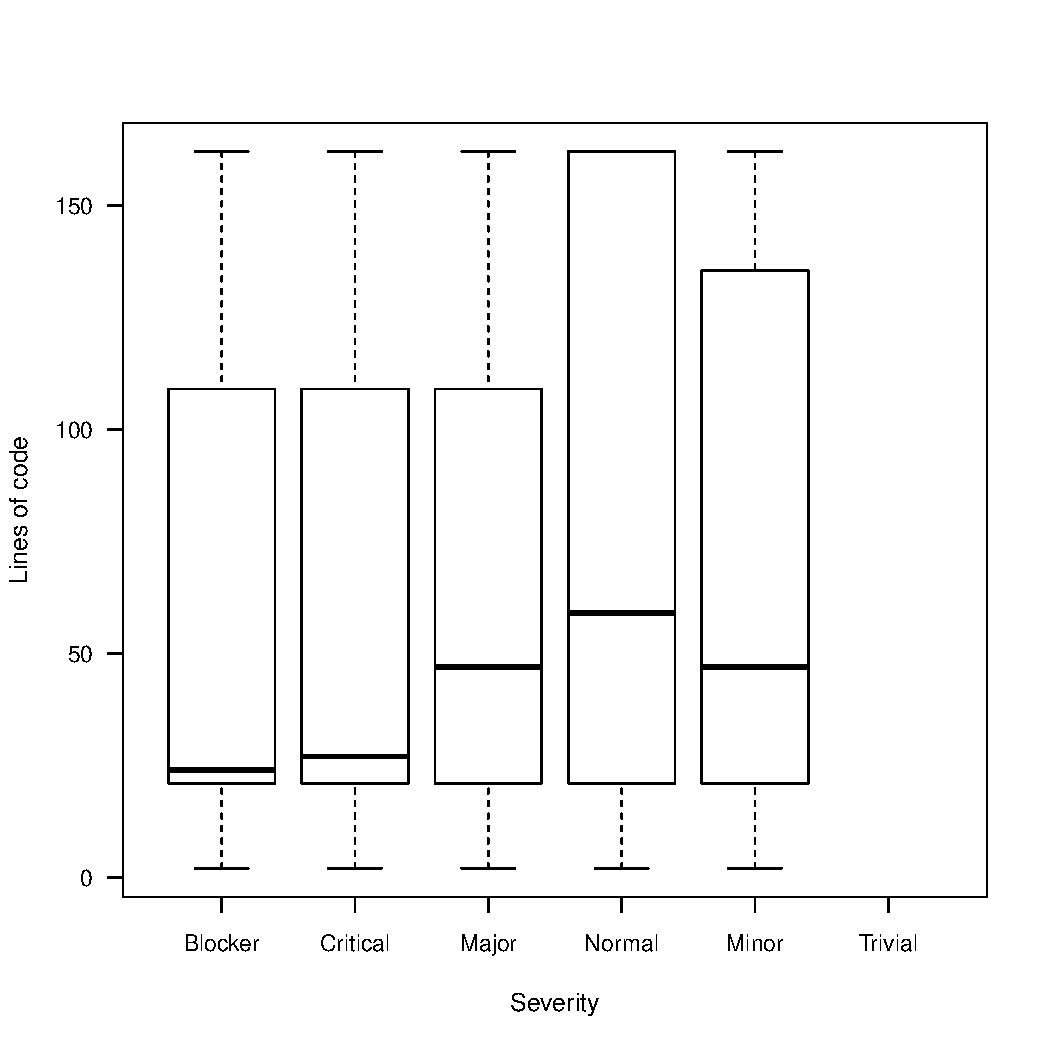
\includegraphics[width=\textwidth]{img/core-classcount-sev-boxplot.pdf}
                \caption{NOC}
                \label{fig:box-sevcore-noc}
        \end{subfigure}%
        ~ %add desired spacing between images, e. g. ~, \quad, \qquad etc. 
          %(or a blank line to force the subfigure onto a new line)
        \begin{subfigure}[b]{0.5\textwidth}
                \centering
                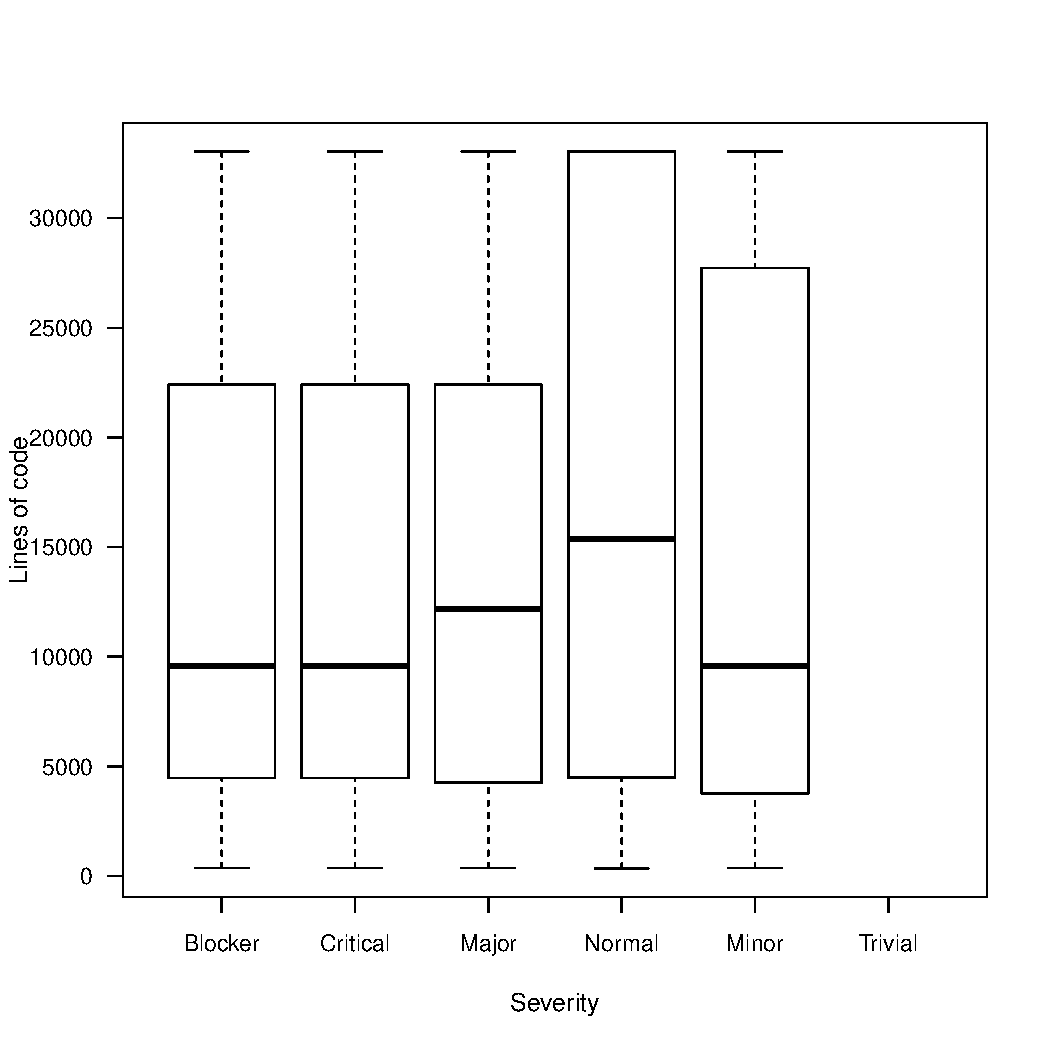
\includegraphics[width=\textwidth]{img/core-loc-sev-boxplot.pdf}
                \caption{SUMLOC}
                \label{fig:box-sevcore-sumloc}
        \end{subfigure}

        \begin{subfigure}[b]{0.5\textwidth}
                \centering
                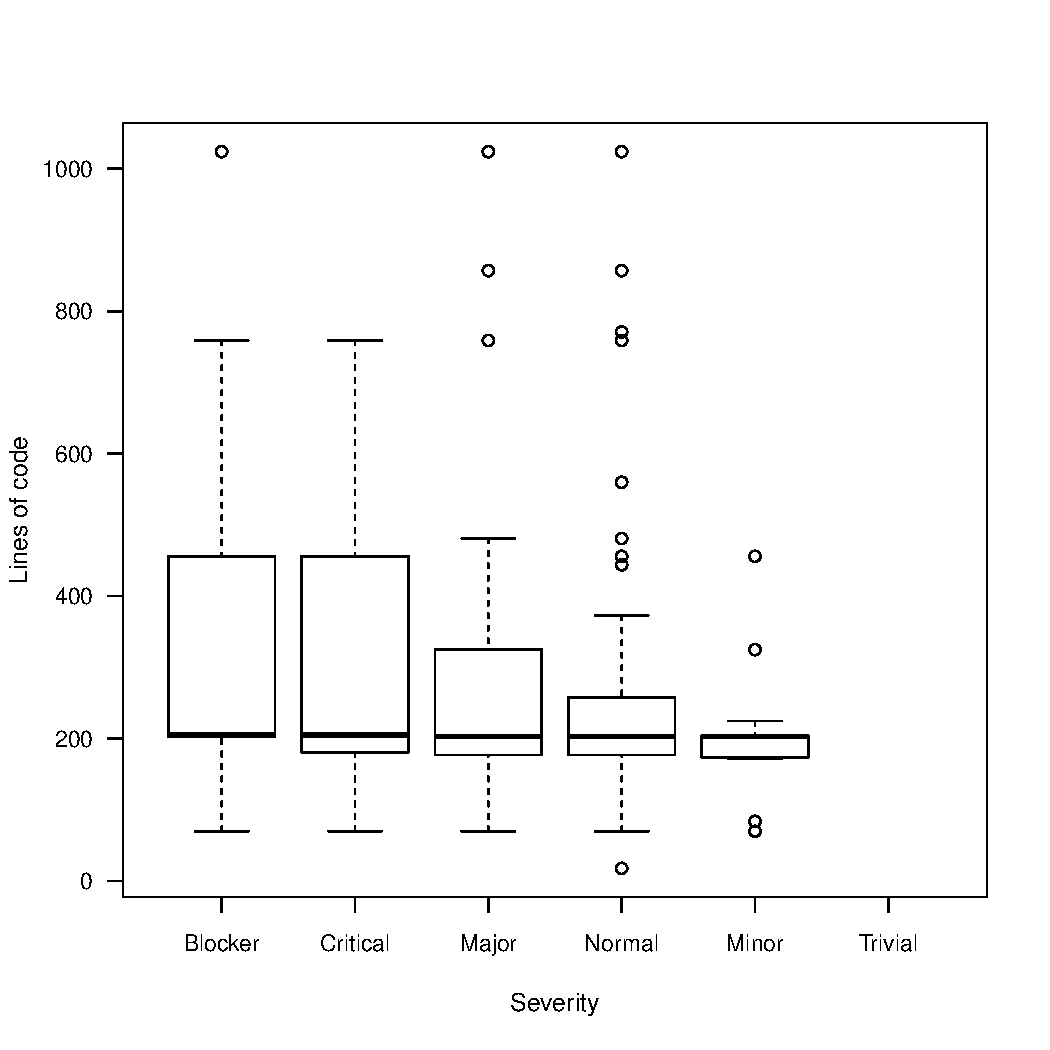
\includegraphics[width=\textwidth]{img/core-avgloc-sev-boxplot.pdf}
                \caption{AVGLOC}
                \label{fig:box-sevcore-avgloc}
        \end{subfigure}
        \caption{Distribution of package size for unique packages that are mentioned in associated bug reports for jdt.core (whiskers at 1.5 times the IQR).}
        \label{fig:packages-box-sevcore}
\end{figure}

\begin{table}[!ht]\footnotesize
	\centering
	\begin{tabular}{lrrrrrr}
		\toprule
		severity & N & min & max & mean & median & std \\
		\midrule
		NOC \\
		\midrule 
		Blocker & 57 & 2 & 162 & 55 & 24 & 52\\
		Critical & 56 & 2 & 162 & 63 & 27 & 54\\
		Major & 180 & 2 & 162 & 69 & 47 & 58\\
		Normal & 859 & 2 & 162 & 77 & 59 & 61\\\\
		\midrule
		SUMLOC \\
		\midrule
		Blocker & 57 & 369 & 33,032 & 13,201 & 9,584 & 10,049\\
		Critical & 56 & 369 & 33,032 & 14,428 & 9,584 & 10,546\\
		Major & 180 & 369 & 33,032 & 15,413 & 12,168 & 11,332\\
		Normal & 859 & 351 & 33,032 & 16,763 & 15,366 & 12,030\\\\
		\midrule
		AVGLOC \\
		\midrule
		Blocker & 57 & 70 & 1,024 & 308 & 205 & 174\\
		Critical & 56 & 70 & 759 & 283 & 205 & 172\\
		Major & 180 & 70 & 1,024 & 275 & 203 & 192\\
		Normal & 859 & 18 & 1,024 & 266 & 203 & 195\\
		\bottomrule
	\end{tabular} 
	\caption{Package size statistics for unique packages that are mentioned in associated bug reports (jdt.core). N is the number of unique packages.}
	\label{tab:package-sev-stats}
\end{table}

Since the data sets are not normal distributed and the distributions of the data sets are similar shaped (see Appendix~\ref{sub:norm:package_size}), a Wilcoxon Rank Sum test (see Section~\ref{sub:wilcoxon_rank_sum_test}) is used to compare the medians of the data sets. The null hypothesis for the Wilcoxon test states that the median values of two data sets does not differ. The alternative hypothesis for the one-sided test states $M_1 > M_2$, where $M_i$ is the median of group $i$. The results of the one-sided Wilcoxon Rank Sum test between the data sets are given in Table~\ref{tab:wilcoxon-package-sevcore}. As can be seen, only for NOC, a significant value is found (major versus normal severity). $p$-values for NOC and SUMLOC tend to be lower than for AVGLOC, with is consistent with the decrease in median and mean values that is shown when the severity becomes higher.

\begin{table}[!ht]\footnotesize
	\centering
	\begin{tabular}{llrl}
		\toprule
		data set 1 & data set 2 & $p$-value & \\
		\midrule
		NOC \\  
		\midrule
		blocker & critical & $0.1717$ & \\
		critical & major & $0.3388$ & \\
		major & normal & $0.0357$ & * \\\\
		\midrule
		SUMLOC \\  
		\midrule
		blocker & critical & $0.3335$ & \\
		critical & major & $0.3262$ & \\
		major & normal & $0.1183$ & \\\\
		\midrule
		AVGLOC \\  
		\midrule
		blocker & critical & $0.8375$ & \\
		critical & major & $0.7658$ & \\
		major & normal & $0.8766$ & \\
		\bottomrule
	\end{tabular} 
	\caption{One-sided Wilcoxon test results.}
	\label{tab:wilcoxon-package-sevcore}
\end{table}
% subsection analysis (end)

\subsection{Conclusions} % (fold)
In this section, a possible relationship between priority (or severity) and package size is investigated. Package size is defined in three ways, as described in the introduction of this section. The hypothesis for this section state that bug reports with a higher priority (or severity) are associated with packages that have a higher median value of the size metric.

Regarding the data sets for priority, the hypothesis can not be investigated due to a lack of data. Therefore,we can not conclude anything about hypothesis H1.3:

\vspace{\baselineskip}
\hypac{}
\vspace{\baselineskip}

\noindent
Also, for severity in the case of \texttt{jdt.debug}, the data is not suitable to investigate the hypothesis. In the case of \texttt{jdt.core}, sufficient data is available for categories `blocker', `critical', `major' and `normal'. The medians of the before mentioned groups are compared pairwise using a Wilcoxon Rank Sum test. The results for this test are shown in Table~\ref{tab:wilcoxon-package-sevcore}. 

Is is shown that for each test performed, the $p$-value is larger than 0.05, except for the `major' versus `normal' comparison for NOC. With these $p$-values, we accept the null hypothesis of the Wilcoxon Rank Sum test for all tests. Therefore, there is some evidence that the medians of the data sets do not differ. This leads to sufficient evidence to reject Hypothesis H1.4:

\vspace{\baselineskip}
\hypad{}
\vspace{\baselineskip}
% subsection conclusions (end)

% section analysis_of_priority_and_severity_related_to_package_size (end)

\section{Analysis of priority and severity related to class size} % (fold)
\label{sec:analysis_of_priority_and_severity_related_to_lines_of_code}
Lines of code of a class is often used as one of the most important metrics for class size. Other metrics, such as number of methods, fan-in, fan-out and depth-in-tree are sometimes also considered.

In this section, we investigate if there is a relation between the priority of a bug report and the lines of code of the corresponding classes referenced in the stack traces in that bug report. Likewise, the investigation will be done for the severity of a bug report. 

In short, the following two hypotheses of research question R1 will be discussed: 

\vspace{\baselineskip}
\hypae{}

\vspace{\baselineskip}
\hypaf{}

\vspace{\baselineskip}

\subsection{Results} % (fold)
For each bug report with a stack trace, all associated classes are determined, which all have a lines of code metric (when the source code can be found in the source code repository). A bug report can have multiple stack traces, and a stack trace can have multiple associated classes. This results in a list of pairs \emph{(report, class)}. It is possible that the same stack trace is mentioned multiple times in a bug report (for example in a quoted message). Also, a class can be mentioned multiple times in a stack trace. 

In order to make sure these duplicates do not affect the statistics, only \emph{unique} pairs \emph{(report, class)} are considered. Table~\ref{tab:loc-stats} shows some descriptive statistics for the lines of code metric of all unique pairs \emph{(report, class)} mentioned in the bug reports. These statistics are also visualised as box plots in Figure~\ref{fig:loc-boxplot}. As can be seen, \texttt{jdt.debug} and \texttt{jdt.core} both have a specific signature when it comes to lines-of-code.

\begin{table}[!ht]\footnotesize
	\centering
	\begin{tabular}{lrrrrrr}
		\toprule
		data set & N & min & max & mean & median & std \\
		\midrule
		\texttt{jdt.debug} & 74 & 13 & 2,623 & 323 & 192 & 419 \\
		\texttt{jdt.core} & 264 & 20 & 10,833 & 688 & 322 & 1,231 \\
		\bottomrule
	\end{tabular} 
	\caption{Lines of code statistics for unique classes that are mentioned in associated bug reports. N is the number of unique classes.}
	\label{tab:loc-stats}
\end{table}

\begin{figure}[!ht]
	\centering
		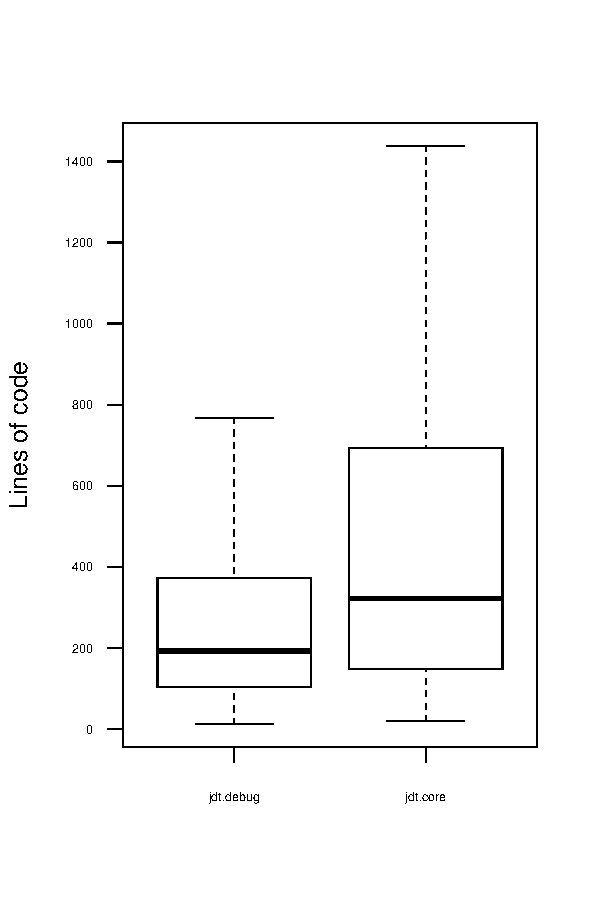
\includegraphics[width=0.7\textwidth]{img/debug-core-loc-mentioned-boxplot.pdf}
	\caption{Lines of code for unique classes that are mentioned in associated bug reports (whiskers at 1.5 times the IQR, outliers not shown).}
	\label{fig:loc-boxplot}
\end{figure}

Regarding the unique pairs \emph{(report, class)}, the tuple counts can be seen in Table~\ref{tab:prio-loc-counts}. Please note the total number of observations is higher than the number of observations in Table~\ref{tab:loc-stats}. This is of course due to the fact that the data is now also grouped on bug report. The corresponding box plots can be seen in Figure~\ref{fig:box-prio-sev}. Both for priority and severity, visually, no distinct pattern can be discovered, although median values do not seem to change much.

\begin{table}[!ht]\footnotesize
	\centering
	\begin{tabular}{lrrrrrr}
		\toprule
		 & \texttt{jdt.debug} &  & \texttt{jdt.core} &  & overall & \\
		 & all & unique & all & unique & all & unique\\
		\midrule
		P1 & 7 & 4 & 31 & 14 & 38 & 18\\
		P2 & 76 & 31 & 56 & 23 & 132 & 54\\
		P3 & 1,639 & 511 & 6,171 & 2,633 & 7,810 & 3,144\\
		P4 & 21 & 8 & 0 & 0 & 21 & 8\\
		P5 & 0 & 0 & 97 & 35 & 97 & 35\\
		\midrule
		Total & 1,743 & 554 & 6,355 & 2,705 & 8,098 & 3,259\\
		\midrule
		\\
		Blocker & 0 & 0 & 281 & 134 & 281 & 134\\
		Critical & 23 & 11 & 274 & 121 & 297 & 132\\
		Major & 348 & 79 & 1,124 & 439 & 1,472 & 518\\
		Normal & 1,329 & 454 & 4,565 & 1,966 & 5,894 & 2,420\\
		Minor & 1 & 1 & 100 & 40 & 101 & 41\\
		Trivial & 7 & 3 & 0 & 0 & 7 & 3\\
		\midrule
		Total & 1,708 & 548 & 6,344 & 2,700 & 8,052 & 3,248\\
		\bottomrule
	\end{tabular} 
	\caption{Unique \emph{(report, class)} pair-counts.}
	\label{tab:prio-loc-counts}
\end{table}

\begin{figure}
        \begin{subfigure}[b]{0.5\textwidth}
                \centering
                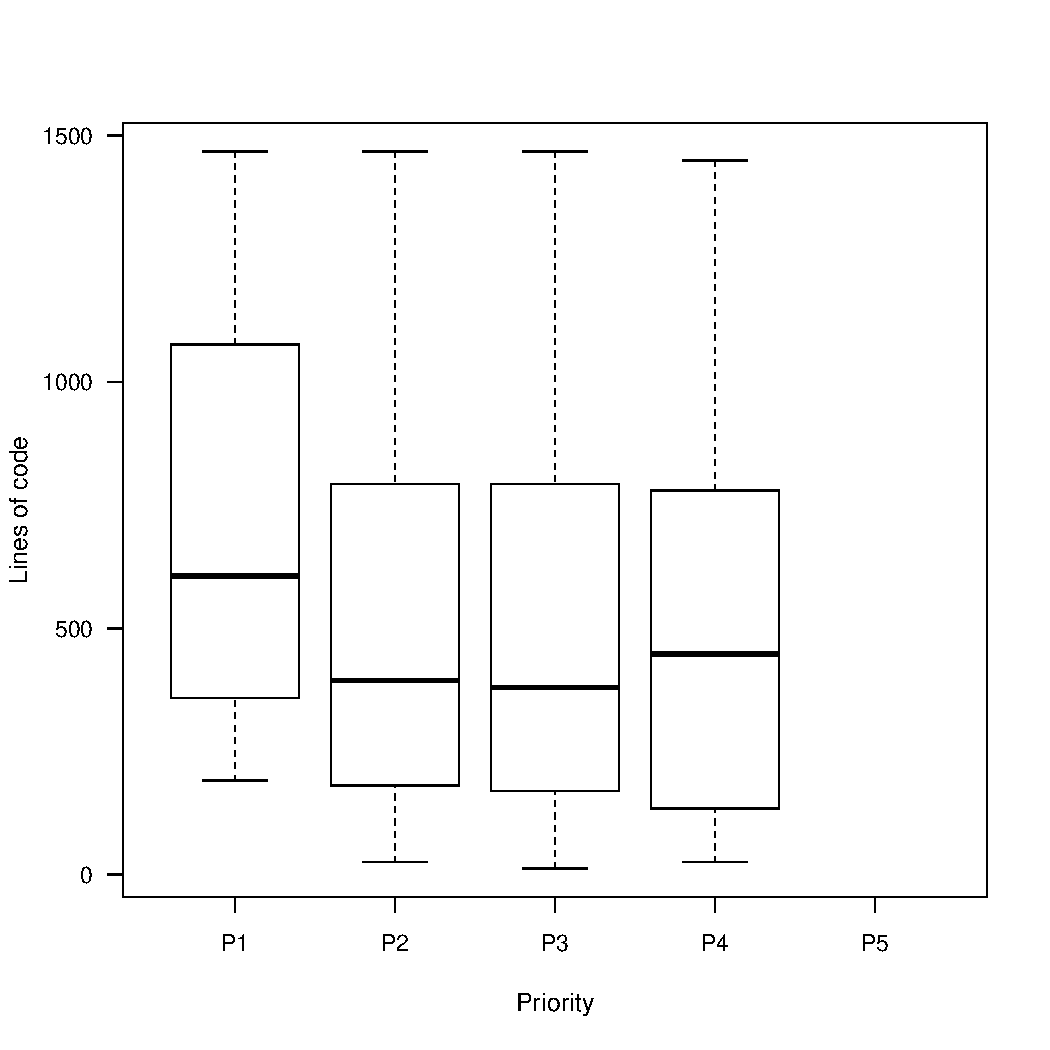
\includegraphics[width=\textwidth]{img/debug-unique-prio-boxplot.pdf}
                \caption{Priority --- jdt.debug}
                \label{fig:box-prio-debug}
        \end{subfigure}%
        ~ %add desired spacing between images, e. g. ~, \quad, \qquad etc. 
          %(or a blank line to force the subfigure onto a new line)
        \begin{subfigure}[b]{0.5\textwidth}
                \centering
                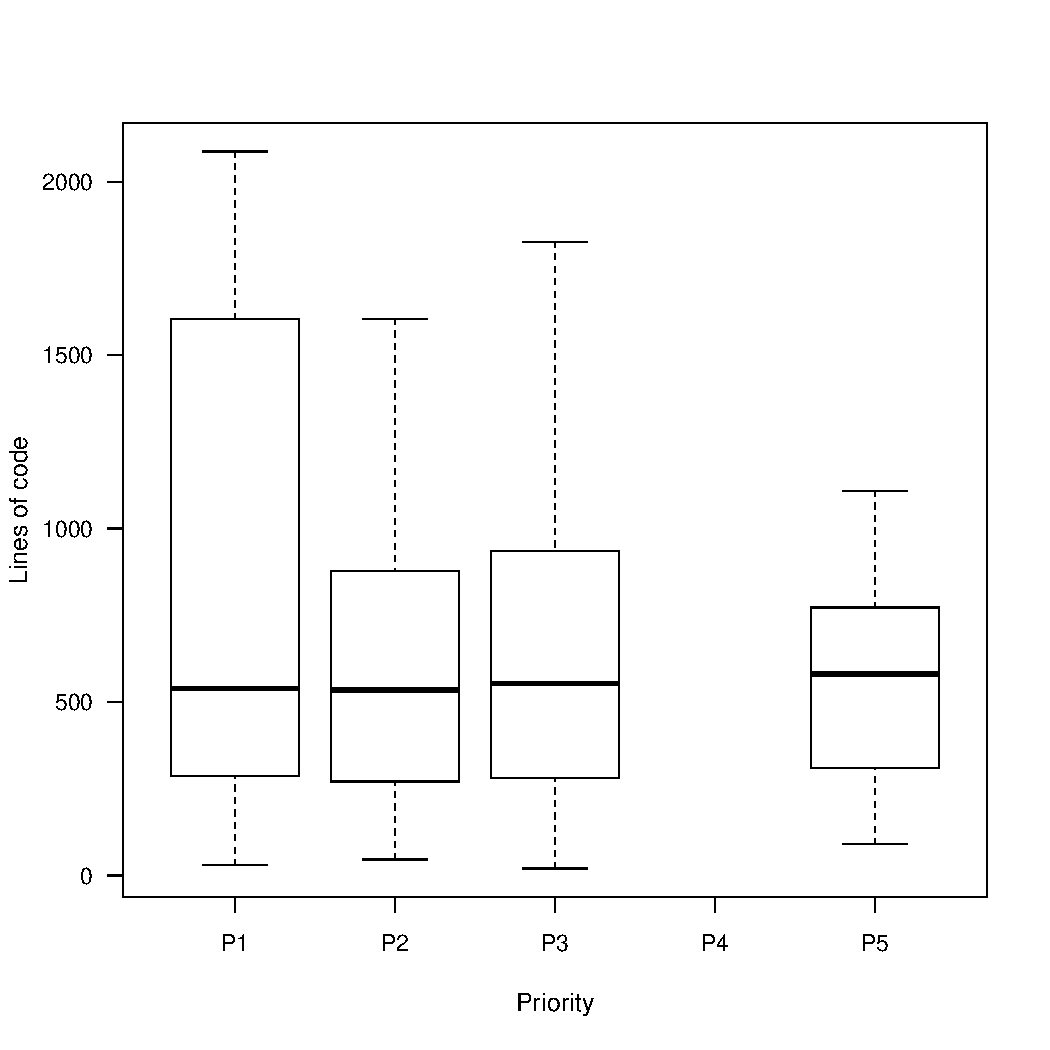
\includegraphics[width=\textwidth]{img/core-unique-prio-boxplot.pdf}
                \caption{Priority --- jdt.core}
                \label{fig:box-prio-core}
        \end{subfigure}

        \begin{subfigure}[b]{0.5\textwidth}
                \centering
                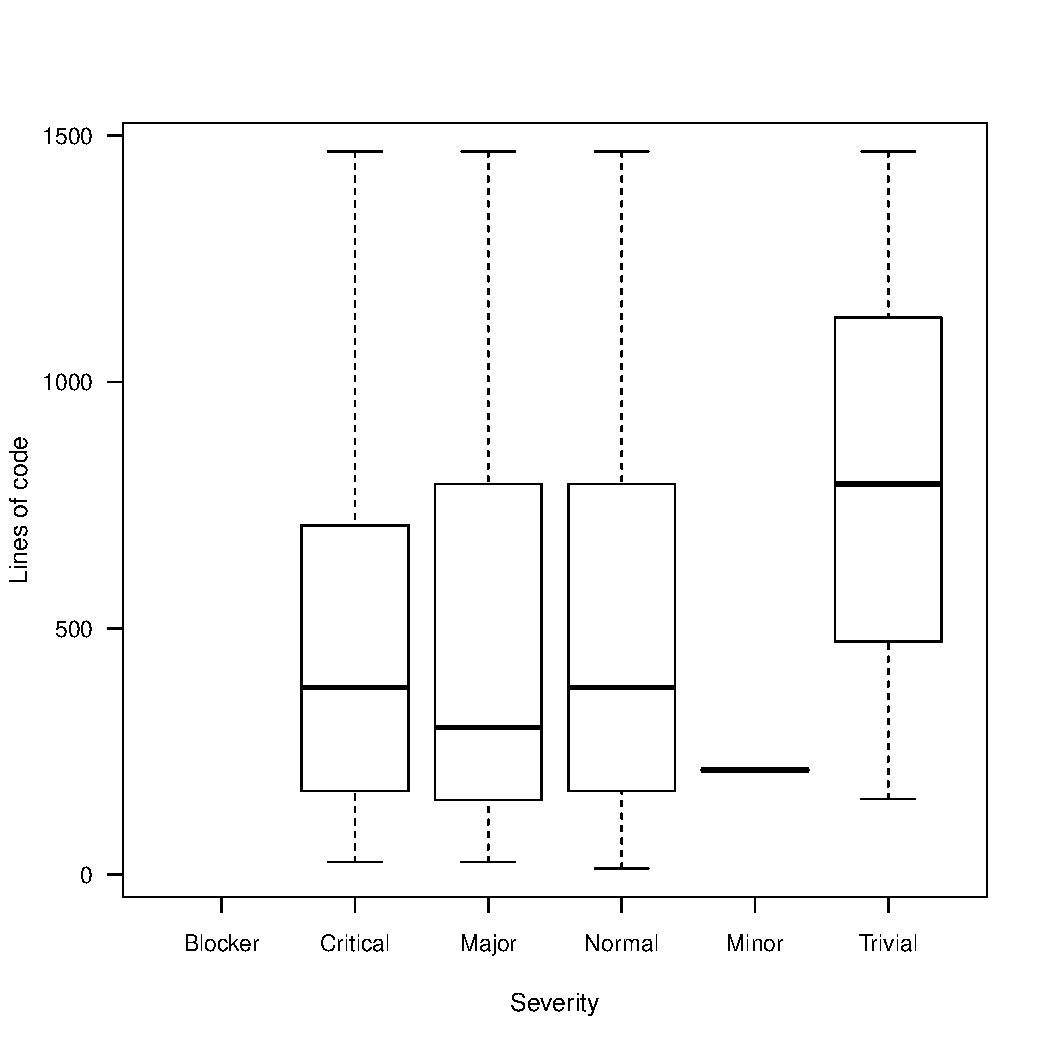
\includegraphics[width=\textwidth]{img/debug-unique-sev-boxplot.pdf}
                \caption{Severity --- jdt.debug}
                \label{fig:box-sev-debug}
        \end{subfigure}
        ~ %add desired spacing between images, e. g. ~, \quad, \qquad etc. 
          %(or a blank line to force the subfigure onto a new line)
        \begin{subfigure}[b]{0.5\textwidth}
                \centering
                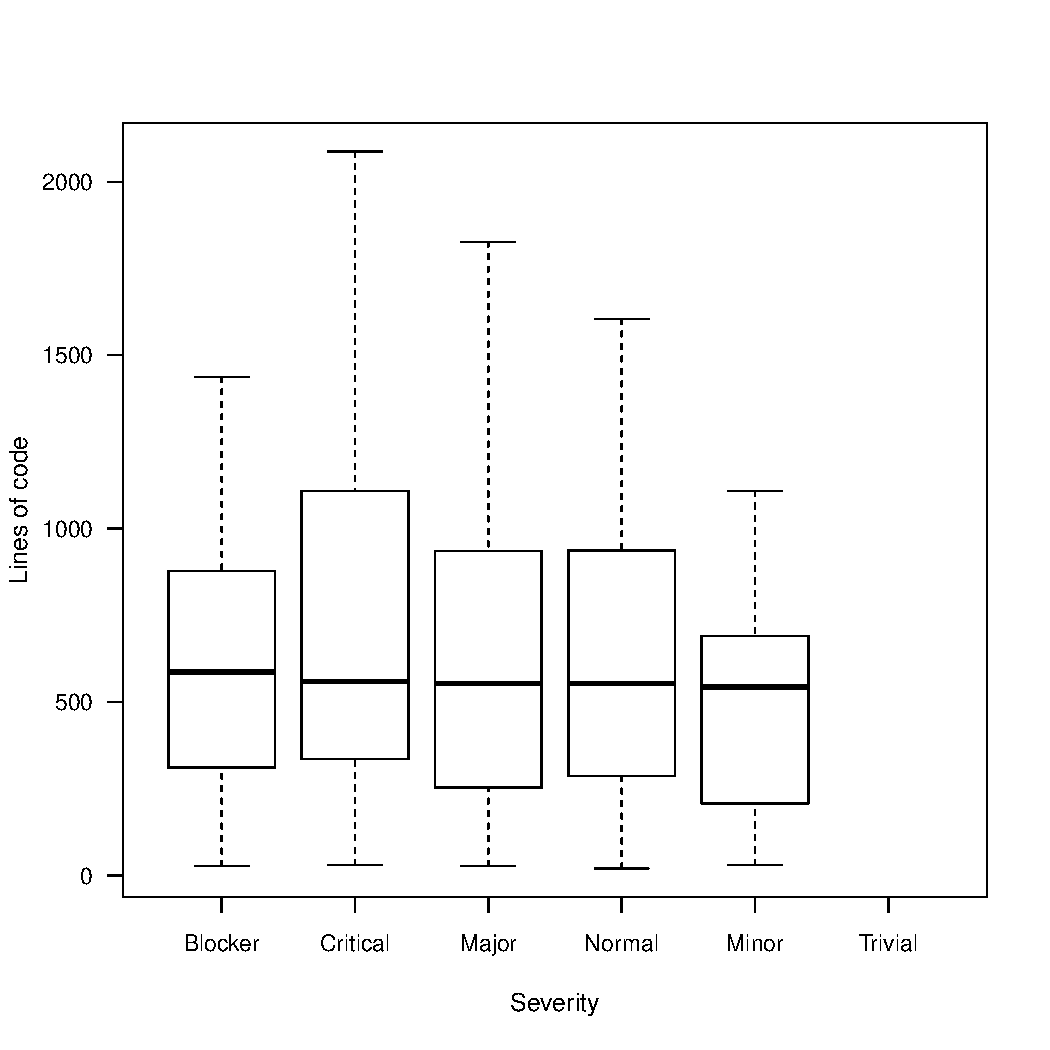
\includegraphics[width=\textwidth]{img/core-unique-sev-boxplot.pdf}
                \caption{Severity --- jdt.core}
                \label{fig:box-sev-core}
        \end{subfigure}
        \caption{Distribution of class size for unique classes that are mentioned in associated bug reports (whiskers at 1.5 times the IQR, outliers not shown).}
        \label{fig:box-prio-sev}
\end{figure}
% subsection results (end)

\subsection{Analysis} % (fold)
In order to investigate whether there is a relation between priority (or severity) and class size, a pairwise comparison of the median values of each data set needs to be made. For priority, P1 and P2 are compared, P2 and P3, et cetera. For severity, `blocker' and `critical' are compared, `critical' and `major', et cetera.

Table~\ref{tab:prio-loc-counts} shows that for \texttt{jdt.debug}, no bug reports with priority P5 are present. The same applies to \texttt{jdt.core} and priority P4. For \texttt{jdt.debug}, the number of data points is also low (4) for priority P1. Regarding the severity, a similar pattern is present. For \texttt{jdt.debug}, a low amount of data points is seen for severities `blocker' (0), `minor' (1) and `trivial' (3), and for \texttt{jdt.core} this applies to `trivial' (0). This is consistent with the research performed in \cite{Lamkanfi2010}, who found that most bug reports get assigned the default value for priority and severity. It is tempting to combine both \texttt{jdt.debug} and \texttt{jdt.core} into one data set to overcome the sample size issues. However, Figure~\ref{fig:loc-boxplot} and Table~\ref{tab:loc-stats} show the distribution of both data sets is quite different. 

This means not all possible pairwise comparisons can be performed. When a minimum sample size of 20 is taken into account, the only logical investigation is the relation between severity and lines of code for the \texttt{jdt.core} project. With this data set, four comparisons can be made (`blocker' vs `critical', `critical' vs `major', `major' vs `normal', `normal' vs `minor'). Using these four comparisons, a possible relationship between the two dimensions (severity and lines of code) can be shown.

The median line of code values of the five datasets for \texttt{jdt.core} are shown in Table~\ref{tab:statistics-invg}. Figure~\ref{fig:box-prio-sev} shows the box plots for the data sets.

\begin{table}[!ht]\footnotesize
	\centering
	\begin{tabular}{lrrrrrr}
		\toprule
		severity & N & min & max & mean & median & std \\
		\midrule
		Blocker & 134 & 27 & 8,218 & 857 & 586 & 1,052\\
		Critical & 121 & 29 & 8,218 & 1,046 & 559 & 1,507\\
		Major & 439 & 27 & 10,833 & 887 & 553 & 1,228\\
		Normal & 1,966 & 20 & 10,833 & 974 & 553 & 1,494\\
		Minor & 40 & 30 & 3,297 & 605 & 544 & 640\\
		\bottomrule
	\end{tabular} 
	\caption{Lines of code statistics for data under investigation (jdt.core). N is the number of measurements.}
	\label{tab:statistics-invg}
\end{table}

Since the data sets are not normally distributed and the distributions of the data sets are similar shaped (see Appendix~\ref{sub:norm:package_size}), a Wilcoxon Rank Sum test (see Section~\ref{sub:wilcoxon_rank_sum_test}) is used to compare the medians of the data sets. The null hypothesis for the Wilcoxon test states that the median values of two data sets does not differ. The alternative hypothesis for the one-sided test states $M_1 > M_2$, where $M_i$ is the median of group $i$. The results of the one-sided Wilcoxon Rank Sum test between the data sets are given in Table~\ref{tab:wilcoxon-sev-core}. The $p$-values do not show any significant results that might lead to suspecting a shift in median time-to-fix, which corresponds with the data shown in Figure~\ref{fig:box-prio-sev}(d).

\begin{table}[!ht]\footnotesize
	\centering
	\begin{tabular}{llrl}
		\toprule
		data set 1 & data set 2 & $p$-value & \\
		\midrule
		blocker & critical & $0.5575$ & \\
		critical & major & $0.8679$ & \\
		major & normal & $0.3497$ & \\
		normal & minor & $0.9094$ & \\
		\bottomrule
	\end{tabular} 
	\caption{One-sided Wilcoxon test results for jdt.core.}
	\label{tab:wilcoxon-sev-core}
\end{table}

% subsection analysis (end)
\subsection{Conclusions} % (fold)
In this section, a possible relationship between priority (or severity) and class size is investigated. As a hypothesis it is stated that bug reports with a higher priority (or severity) are associated with classes mentioned in bug report stack traces that have a higher median value of the lines of code metric.

Regarding the data sets for priority, the hypothesis can not be investigated due to a lack of data. Therefore, we cannot conclude anything about hypothesis H1.5:

\vspace{\baselineskip}
\hypae{}
\vspace{\baselineskip}

\noindent
Also, for severity in the case of \texttt{jdt.debug}, the data is also not suitable to investigate the hypothesis. For severity in the case of \texttt{jdt.core}, sufficient data is available for categories `blocker', `critical', `major', `normal' and `minor'. The medians of the before mentioned groups are compared pairwise using a Wilcoxon Rank Sum test. The results for this test are shown in Table~\ref{tab:wilcoxon-sev-core}. Is is shown that for each test performed, the $p$-value is larger than 0.05. With these $p$-values, we accept the null hypothesis of the Wilcoxon Rank Sum test for all tests. Therefore, there is no evidence that the medians of the data sets differ. We therefore reject hypothesis H1.6:

\vspace{\baselineskip}
\hypaf{}
\vspace{\baselineskip}
 
% subsection conclusions (end)

% section analysis_of_priority_and_severity_related_to_lines_of_code (end)

\section{Summary of results} % (fold)
\label{sec:priosev-summary_of_results}
This chapter showed the results and analysis for research question R1, as described in Chapter~\ref{sec:analysis:priority_and_severity}:

\vspace{\baselineskip}
\questiona{}
\vspace{\baselineskip}

\noindent
First, it was investigated whether the presence of one or more stack traces in a bug report corresponds with a higher priority (or severity) of the bug report. For priority, some evidence is found for \texttt{jdt.debug}, with strong evidence for \texttt{jdt.core}. This gives enough evidence to partially accept hypothesis H1.1. For severity, the number of bug reports with a higher than normal severity increases when a stack trace is present. Also, the number of bug reports with a lower than normal severity decreases when a stack trace is present. Therefore hypothesis H1.2 is accepted.

The second investigation is about a possible relation between priority (and severity) and package size. Three definitions of package size are investigated. For priority, not enough data is present, so it is not possible to state anything regarding hypothesis H1.3. For severity, sufficient data is only available for \texttt{jdt.core}. For this case, there is no evidence of a relation between severity and package size. Concluding, there is some evidence to reject hypothesis H1.4.

Finally, the second investigation is repeated for a finer granularity: class size. For priority, there is no sufficient data available. Therefore it is not possible to state anything regarding hypothesis H1.5. For severity, sufficient data is available for \texttt{jdt.core}, but there is no evidence that the medians of the data sets differ. Concluding, there is some evidence to reject hypothesis H1.6.

The next chapter investigates whether there is a relation between bug reports and the time-to-fix of a bug.
% section summary_of_results (end)
% chapter results_priority_and_severity (end)